\documentclass[11pt]{article}
\usepackage{graphicx}
\usepackage{amsmath}
\usepackage{hyperref}
\usepackage{listings}


\topmargin=-0.45in
\evensidemargin=0in
\oddsidemargin=0in
\textwidth=6.5in
\textheight=9.0in
\headsep=0.25in
\renewcommand{\thesubsection}{\alph{subsection})}
\renewcommand\lstlistingname{Snippet}
\renewcommand\lstlistlistingname{}

\usepackage{xcolor}
\definecolor{codegreen}{rgb}{0,0.6,0}
\definecolor{codegray}{rgb}{0.5,0.5,0.5}
\definecolor{codeorange}{rgb}{1,0.49,0}
\definecolor{backcolour}{rgb}{0.95,0.95,0.96}

\lstdefinestyle{mystyle}{
    backgroundcolor=\color{backcolour},   
    commentstyle=\color{codegray},
    keywordstyle=\color{codeorange},
    numberstyle=\tiny\color{codegray},
    stringstyle=\color{codegreen},
    basicstyle=\ttfamily\footnotesize,
    breakatwhitespace=false,         
    breaklines=true,                 
    captionpos=b,                    
    keepspaces=true,                 
    numbers=left,                    
    numbersep=5pt,                  
    showspaces=false,                
    showstringspaces=false,
    showtabs=false,                  
    tabsize=2,
    xleftmargin=10pt,
}

\lstset{style=mystyle}
% Title and Author Customization

% --------------------
% Start from here
% --------------------

\title{
    \vspace{3em}
    \textbf{Digital Signal Processing Lab}\\
    Demo 4 - Exercise 2 (Matlab GUI)
    \vspace{1em}
}
\author{
    Saad Zubairi \\ 
    shz2020 \\
    \vspace{1em}
}
\vspace{1em}
\date{September 24th, 2025}

\begin{document}
\maketitle	

\pagebreak

% --------------------
% Body
% --------------------


\section*{Solution}

This solution contains a Matlab GUI app script that lets us visualize a low pass filter along with the pertaining Frequency Response (Magnitude) and the impulse response of the filter. The solution uses the uifigure function to add multiple ui elements such as a nested plot (which contains all the three plots) and a slider that controls the cut-off frequency. 

Key changes made from the included file:

\begin{itemize}
    \item A subplot has been added (using \texttt{uigridlayout} function)
    \begin{lstlisting}[language=matlab, label={lst:code}, breaklines=true, caption={plot changes}]
    % grid layout
    grid = uigridlayout(my_fig,[3 1]); 
    grid.RowHeight = {'1x', 'fit', 'fit'}; 
    grid.ColumnWidth = {'1x'};

    % sub-grid for plots
    plots = uigridlayout(grid,[1 3]);
    plots.RowHeight   = {'1x'};
    plots.ColumnWidth = {'1x','1x','1x'};
    \end{lstlisting}
    

    \item The cut off frequency is controlled in a state variable defined as:

    \begin{lstlisting}[language=matlab, label={lst:code}, breaklines=true, caption={state variable}]
    fc = slider.Value;
    update_plot()
    \end{lstlisting}
    
    \item The \texttt{update\char`_graph} function accomodates the additional two graphs
    
    \begin{lstlisting}[language=matlab, label={lst:code}, breaklines=true, caption={state variable}]
    function update_plot()
        % design
        [b,a]=butter(2,2*fc); 
        y=filtfilt(b,a,x); 

        % time
        set(line_handle,'YData',y);

        % |H(f)| dB
        Nfft = 2048;
        [H,w]=freqz(b,a,Nfft,'half'); f=w/(2*pi);
        magdB = 20*log10(max(abs(H),1e-6));

        set(freq_line,'XData',f,'YData',magdB); ax2.Children(1).Value = fc;
        title(ax2,'|H(f)| (dB)');

        % h[n]
        Lh=128; h=filter(b,a,[1 zeros(1,Lh-1)]);
        set(imp_line,'XData',0:Lh-1,'YData',h); xlim(ax3,[0 Lh-1]); title(ax3,'Impulse response h[n]');
    end
    \end{lstlisting}   

\end{itemize}

\section*{Screenshots}

\begin{center}
    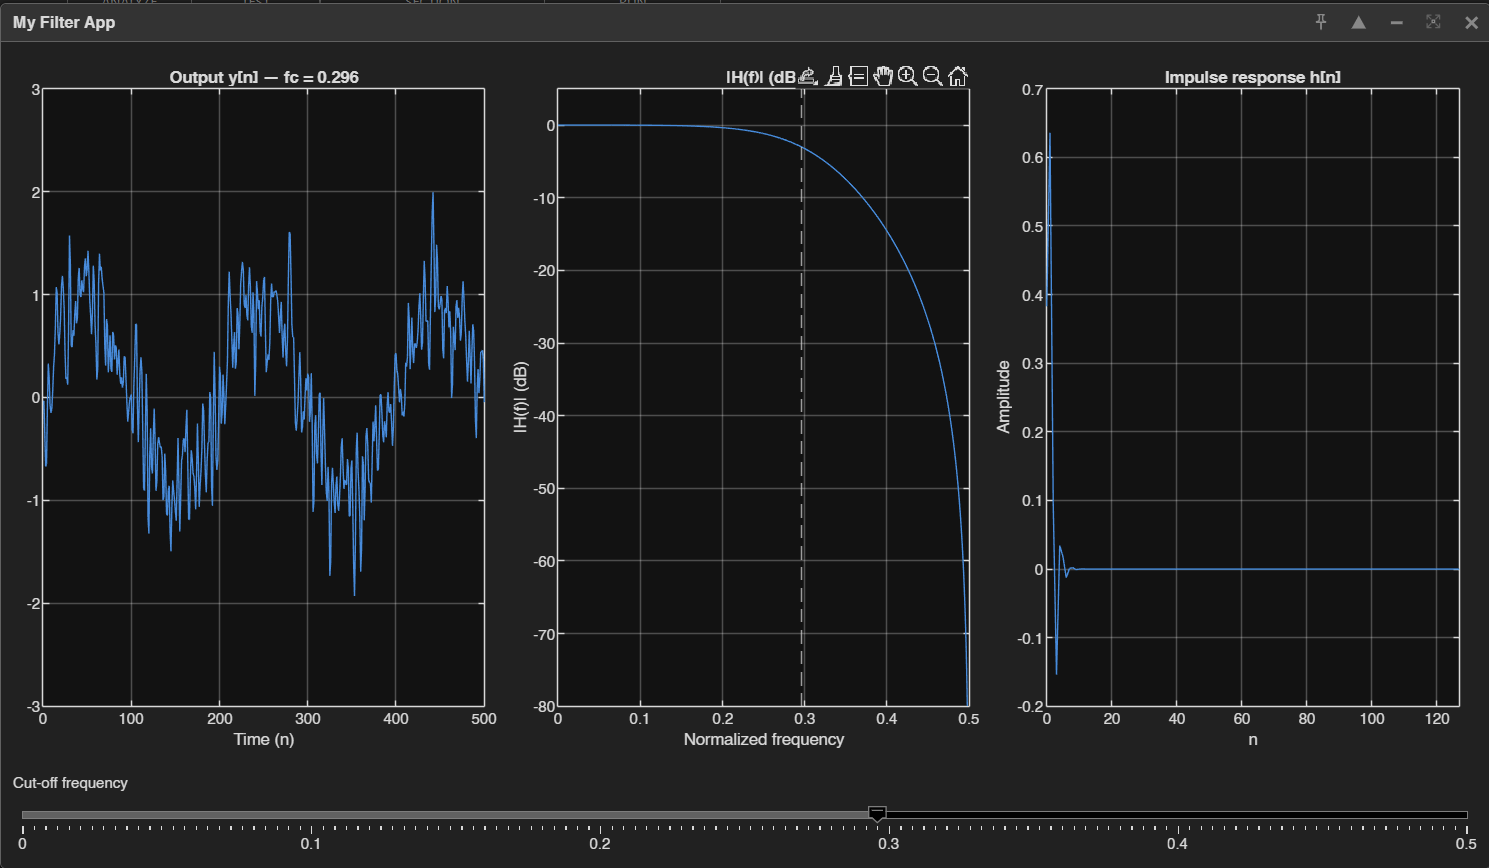
\includegraphics[scale=0.4]{SS1.png}
\end{center}
\begin{center}
    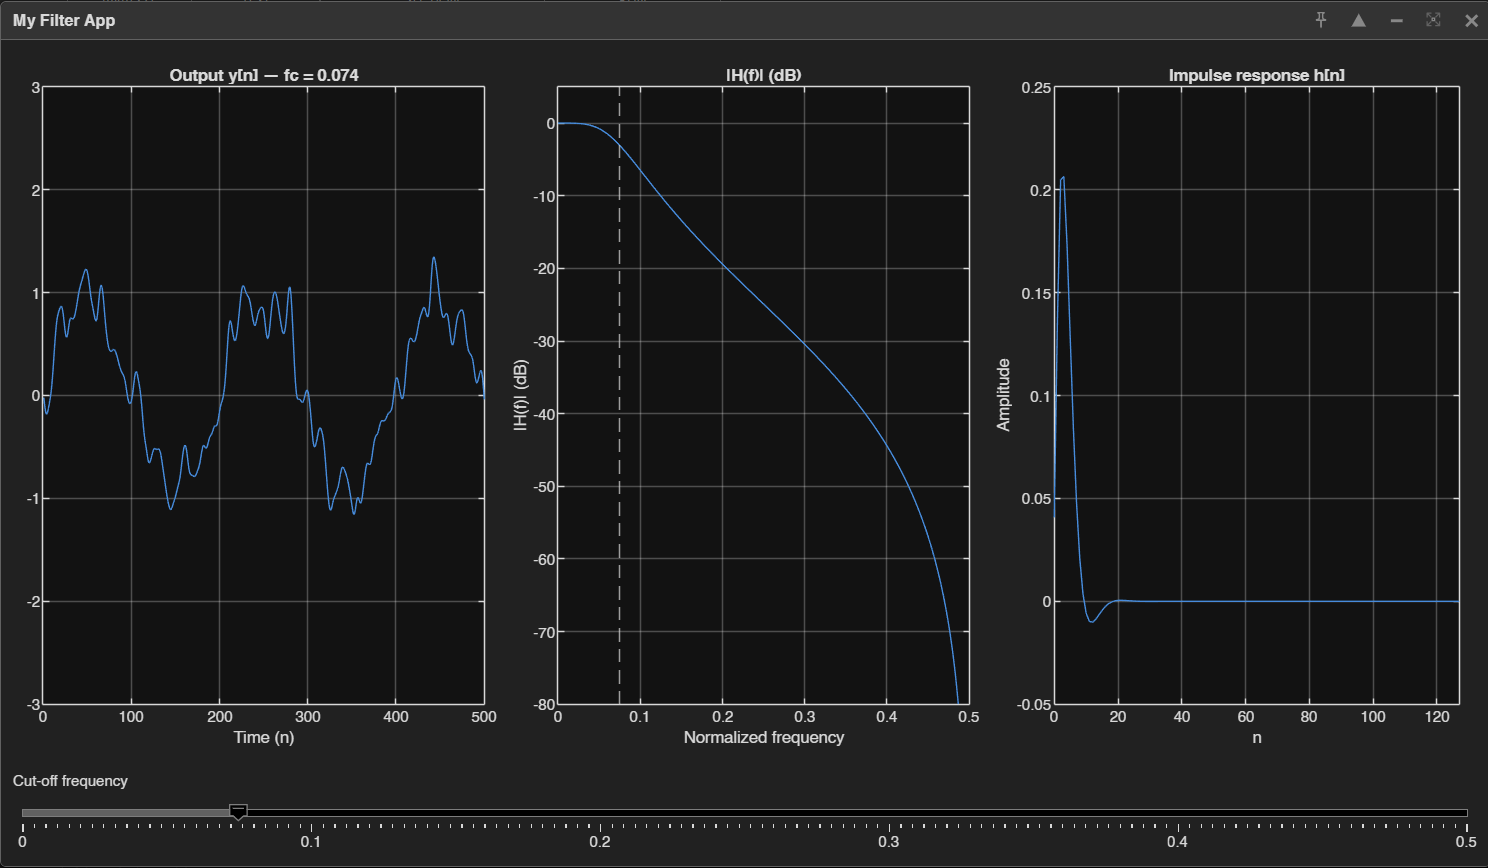
\includegraphics[scale=0.4]{SS2.png}
\end{center}

\pagebreak

\section*{Code}

\begin{lstlisting}[language=matlab, label={lst:code}, breaklines=true, caption={example code}]
function filter_app_ver2

% Set up figure and controls
my_fig = uifigure('Name',"My Filter App");
movegui(my_fig,'center');

% grid layout
grid = uigridlayout(my_fig,[3 1]); 
grid.RowHeight = {'1x', 'fit', 'fit'}; 
grid.ColumnWidth = {'1x'};

% sub-grid for plots
plots = uigridlayout(grid,[1 3]);
plots.RowHeight   = {'1x'};
plots.ColumnWidth = {'1x','1x','1x'};

% Axes
ax  = uiaxes(plots);
ax.XGrid='on'; ax.YGrid='on'; xlabel(ax,'Time (n)'); xlim(ax,[0 500]); ylim(ax,[-3 3]); box(ax,'on')

ax2 = uiaxes(plots);
ax2.XGrid='on'; ax2.YGrid='on'; xlabel(ax2,'Normalized frequency'); ylabel(ax2,'|H(f)| (dB)');
xlim(ax2,[0 .5]); ylim(ax2,[-80 5]); box(ax2,'on')

ax3 = uiaxes(plots);
ax3.XGrid='on'; ax3.YGrid='on'; xlabel(ax3,'n'); ylabel(ax3,'Amplitude'); box(ax3,'on')

% Slider
slider_label = uilabel(grid);
slider_label.Text = 'Cut-off frequency';

slider = uislider(grid);
slider.Value = 0.3;
slider.Limits = [0 0.5];
slider.MajorTicks = 0:0.10:0.5;
slider.ValueChangingFcn = @slider_callback; 

% Signal
N = 500; n = 1:N; x = sin(5*pi*n/N) + 0.5*randn(1,N);

line_handle = line(ax,n,x);

freq_line = plot(ax2,nan,nan); hold(ax2,'on')
xline(ax2,slider.Value,'--'); hold(ax2,'off')

imp_line  = plot(ax3,nan,nan);

% state
fc = slider.Value;
update_plot()

    function slider_callback(~,evt)
        fc = max(0.01,min(0.49,evt.Value));
        update_plot()
    end

    function update_plot()
        % design
        [b,a]=butter(2,2*fc); 
        y=filtfilt(b,a,x); 

        % time
        set(line_handle,'YData',y); 

        % |H(f)| dB
        Nfft = 2048;
        [H,w]=freqz(b,a,Nfft,'half'); f=w/(2*pi);
        magdB = 20*log10(max(abs(H),1e-6));

        set(freq_line,'XData',f,'YData',magdB); ax2.Children(1).Value = fc;
        title(ax2,'|H(f)| (dB)');

        % h[n]
        Lh=128; h=filter(b,a,[1 zeros(1,Lh-1)]);
        set(imp_line,'XData',0:Lh-1,'YData',h); xlim(ax3,[0 Lh-1]); title(ax3,'Impulse response h[n]');
    end
end

\end{lstlisting}    




\end{document}